\section{Results}\label{s:6}

We evaluate the trained Deep Q-Network agent (\texttt{dqn\_agent}) against the pre-timed baseline (\texttt{fixed\_time}) on the six held-out test scenarios in the \texttt{TE} split of \texttt{selected\_scenario.csv}, using deterministic action selection ($\arg\max_a Q_\theta(\mathbf{s}_t, a)$) with matched random seed~$42$, control interval $\Delta t = 5\,\mathrm{s}$, minimum green duration $t_{\min} = 10\,\mathrm{s}$, yellow clearance $t_{\text{yellow}} = 3\,\mathrm{s}$, and evaluation horizon $T_{\text{eval}} = 100\,\mathrm{s}$ (20 control steps per episode). The six \texttt{TE} scenarios represent challenging difficulty-level~3 traffic regimes at the Ly Thai To roundabout: complete leg closure and diversion (\texttt{30\_vip\_motorcade\_diversion}, $A_1 = 0$), severe multi-leg saturation (\texttt{49\_extreme\_overload\_all\_legs}, 23{,}000~veh/h aggregate demand), flooding with elevated four-wheel share (\texttt{64\_flooding\_dbp\_reduced}, 39.8\% cars/MPVs/buses/trucks), holiday return surge (\texttt{68\_tet\_return\_flood}), concentrated event dispersal (\texttt{77\_concert\_event\_district3}), and multi-ambulance emergency surges (\texttt{80\_emergency\_multi\_ambulance}, 8.0\% emergency vehicles).

\subsection{Queue Length, Throughput, and Trip-Level Metrics}

Table~\ref{tab:te_primary_results} reports the episode-level comparison between \texttt{dqn\_agent} and \texttt{fixed\_time} across the six \texttt{TE} scenarios, and Fig.~\ref{fig:queue-comparison} visualizes the average instantaneous queue length across all test cases. Note that per-vehicle waiting time, time loss, and travel time are parsed from SUMO's \texttt{tripinfo.xml} output (reflecting vehicles that completed their traversal within $100\,\mathrm{s}$), whereas queue length is averaged over every $5\,\mathrm{s}$ simulation step across all active vehicles.

\begin{table*}[t]
\caption{Episode-level performance comparison between \texttt{dqn\_agent} and \texttt{fixed\_time} across the six \texttt{TE} scenarios ($T_{\text{eval}}=100\,\mathrm{s}$, seed~$42$). Positive percentages ($\Delta\%$) indicate improvement over \texttt{fixed\_time}.}
\label{tab:te_primary_results}
\centering
\scriptsize
\begin{tabular}{lcccccccccccc}
\toprule
\textbf{Scenario ID} & \multicolumn{3}{c}{\textbf{Avg. Queue (veh)}} & \multicolumn{3}{c}{\textbf{Throughput (veh/h)}} & \multicolumn{3}{c}{\textbf{Wait Time$^\dagger$ (s)}} & \multicolumn{2}{c}{\textbf{Time Loss$^\dagger$ (s)}} & \textbf{Switch Rate} \\
\cmidrule(lr){2-4}\cmidrule(lr){5-7}\cmidrule(lr){8-10}\cmidrule(lr){11-12}\cmidrule(lr){13-13}
 & DQN & FT & $\Delta\%$ & DQN & FT & $\Delta\%$ & DQN & FT & $\Delta\%$ & DQN & FT & DQN / FT \\
\midrule
\texttt{30\_vip\_motorcade\_diversion}  & \textbf{21.60} & 27.90 & +22.58 & \textbf{4428.0} & 4356.0 & +1.65  & \textbf{3.03} & 3.99 & +24.03 & \textbf{10.71} & 12.16 & 0.50 / 0.00 \\
\texttt{49\_extreme\_overload\_all\_legs}& \textbf{49.95} & 53.35 & +6.37  & 6012.0 & \textbf{6516.0} & -7.73  & \textbf{2.26} & 2.51 & +10.00 & \textbf{10.14} & 10.73 & 0.75 / 0.00 \\
\texttt{64\_flooding\_dbp\_reduced}     & \textbf{28.70} & 43.50 & +34.02 & \textbf{2844.0} & 2520.0 & +12.86 & 4.82 & \textbf{3.54} & -36.13 & 14.92 & \textbf{11.22} & 0.65 / 0.00 \\
\texttt{68\_tet\_return\_flood}         & \textbf{37.65} & 49.85 & +24.47 & \textbf{5544.0} & 4644.0 & +19.38 & 4.08 & \textbf{2.19} & -85.88 & 13.33 & \textbf{9.86}  & 0.50 / 0.00 \\
\texttt{77\_concert\_event\_district3}  & 31.60 & \textbf{30.70} & -2.93  & 4680.0 & \textbf{4968.0} & -5.80  & 2.46 & \textbf{2.12} & -15.94 & \textbf{10.17} & 10.79 & 0.35 / 0.00 \\
\texttt{80\_emergency\_multi\_ambulance}& \textbf{23.25} & 40.35 & +42.38 & \textbf{4068.0} & 3960.0 & +2.73  & \textbf{3.71} & 3.85 & +3.80  & 12.92 & \textbf{11.76} & 0.70 / 0.00 \\
\midrule
\textbf{Overall Average}                & \textbf{32.12} & 40.94 & +21.15 & \textbf{4596.0} & 4494.0 & +3.85  & 3.39 & \textbf{3.03} & -16.69 & 12.03 & \textbf{11.09} & 0.58 / 0.00 \\
\bottomrule
\end{tabular}
\begin{minipage}{\textwidth}
\vspace{2pt}
\footnotesize
\textit{$^\dagger$Waiting time and time loss are computed from SUMO \texttt{tripinfo.xml} records of vehicles completing traversal within $100\,\mathrm{s}$; see Table~\ref{tab:te_step_and_env} and Section~\ref{s:7} for step-level network-wide delay. Minimum-green violations were $0$ for both controllers in every scenario. Overall Average $\Delta\%$ reports the unweighted mean of the six scenario-level percentages.}
\end{minipage}
\end{table*}

\begin{figure}[t]
\centering
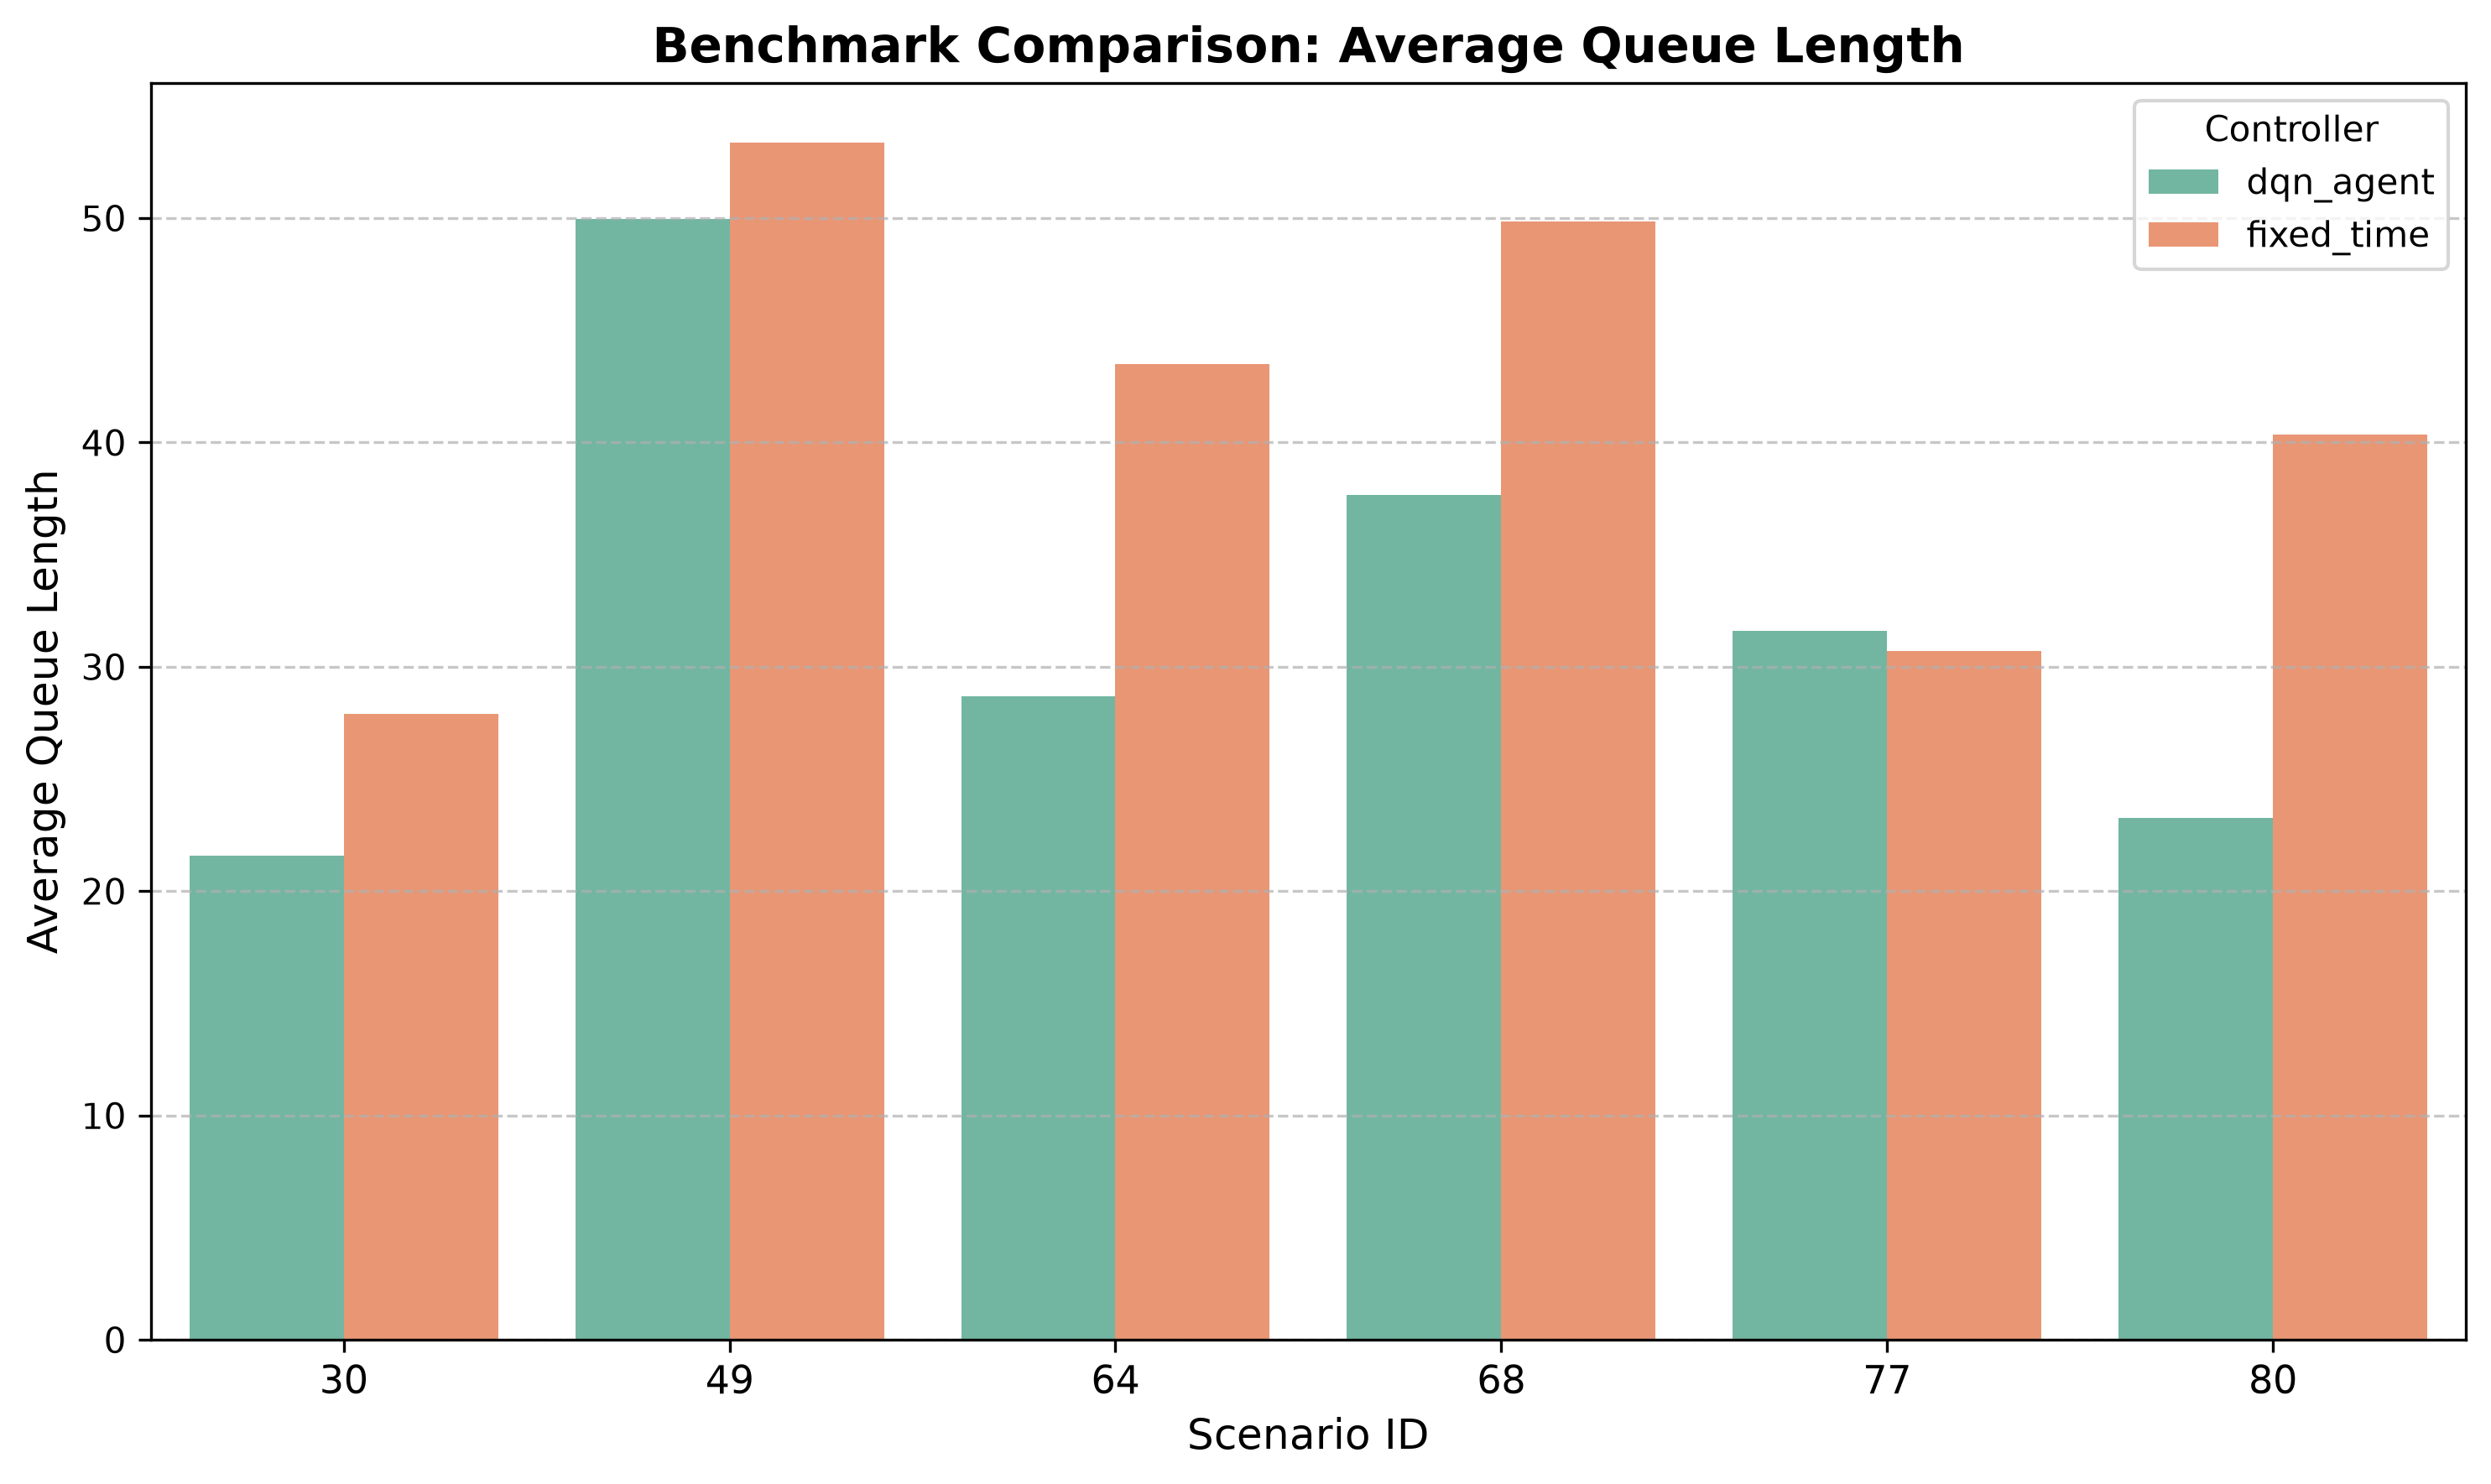
\includegraphics[width=\columnwidth]{figures/queue_comparison.png}
\caption{Average instantaneous queue length comparison between \texttt{dqn\_agent} and \texttt{fixed\_time} across the six \texttt{TE} scenarios (labeled by scenario prefix ID).}
\label{fig:queue-comparison}
\end{figure}

Across the six test scenarios, \texttt{dqn\_agent} reduces mean queue length from $40.94$ to $32.12$ halted vehicles per step, achieving an average improvement of $21.15\%$ ($-8.82$ vehicles). Queue reductions are observed in five of the six scenarios, with the largest gains in \texttt{80\_emergency\_multi\_ambulance} ($42.38\%$, $23.25$ vs.\ $40.35$ vehicles), \texttt{64\_flooding\_dbp\_reduced} ($34.02\%$, $28.70$ vs.\ $43.50$ vehicles), \texttt{68\_tet\_return\_flood} ($24.47\%$, $37.65$ vs.\ $49.85$ vehicles), and \texttt{30\_vip\_motorcade\_diversion} ($22.58\%$, $21.60$ vs.\ $27.90$ vehicles). Only \texttt{77\_concert\_event\_district3} shows a slight queue increase ($31.60$ vs.\ $30.70$ vehicles, $-2.93\%$).

Network throughput improves by $3.85\%$ on average ($4596.0$ vs.\ $4494.0\,\mathrm{veh/h}$), driven by substantial discharge gains under heavy disruption in Scenario~68 ($+19.38\%$, $5544.0$ vs.\ $4644.0\,\mathrm{veh/h}$) and Scenario~64 ($+12.86\%$, $2844.0$ vs.\ $2520.0\,\mathrm{veh/h}$). Under uniform extreme overload (Scenario~49) and event dispersal (Scenario~77), \texttt{fixed\_time} completes more short-horizon trips ($-7.73\%$ and $-5.80\%$ throughput difference). Meanwhile, completed-trip waiting time and time loss in \texttt{tripinfo.xml} favor \texttt{dqn\_agent} in Scenarios~30 ($+24.03\%$ waiting, $+11.87\%$ time loss) and~49 ($+10.00\%$ waiting, $+5.56\%$ time loss), but appear higher for \texttt{dqn\_agent} in Scenarios~64 ($-36.13\%$) and~68 ($-85.88\%$), resulting in an overall completed-trip average of $3.39\,\mathrm{s}$ vs.\ $3.03\,\mathrm{s}$ waiting time and $12.03\,\mathrm{s}$ vs.\ $11.09\,\mathrm{s}$ time loss (and $54.44\,\mathrm{s}$ vs.\ $51.34\,\mathrm{s}$ travel time).

\subsection{Step-Level Network Dynamics, Safety, and Environmental Impact}

To evaluate all active vehicles continuously rather than only completed trips, Table~\ref{tab:te_step_and_env} summarizes the $5\,\mathrm{s}$ step-level telemetry alongside fuel, emissions, and inference latency. Figure~\ref{fig:step-dashboard-64} illustrates the full four-panel dynamic trajectory for Scenario~64 (\texttt{64\_flooding\_dbp\_reduced}).

\begin{table*}[t]
\caption{Step-level network dynamics ($0\text{--}100\,\mathrm{s}$), environmental comparison, and inference latency across the six \texttt{TE} scenarios. Positive percentages in \textbf{Red.} and $\Delta\%$ (Impr.) denote improvement over \texttt{fixed\_time} (lower delay, fuel, or $\mathrm{NO}_x$); negative values denote increases.}
\label{tab:te_step_and_env}
\centering
\scriptsize
\begin{tabular}{lcccccccccc}
\toprule
\textbf{Scenario ID} & \multicolumn{3}{c}{\textbf{Accum. Wait at $100\,\mathrm{s}$ (s)}} & \multicolumn{2}{c}{\textbf{Mean Speed (m/s)}} & \multicolumn{2}{c}{\textbf{Cum. Reward}} & \textbf{Fuel $\Delta\%$} & \textbf{$\mathrm{NO}_x$ $\Delta\%$} & \textbf{Latency (ms)} \\
\cmidrule(lr){2-4}\cmidrule(lr){5-6}\cmidrule(lr){7-8}\cmidrule(lr){9-9}\cmidrule(lr){10-10}\cmidrule(lr){11-11}
 & DQN & FT & Red. (\%) & DQN & FT & DQN & FT & (Impr.) & (Impr.) & DQN \\
\midrule
\texttt{30\_vip\_motorcade\_diversion}  & \textbf{4793}  & 10037 & 52.25\% & \textbf{10.13} & 9.75 & \textbf{-1665} & -1867 & -0.17\% & +1.29\% & 0.529 \\
\texttt{49\_extreme\_overload\_all\_legs}& \textbf{14665} & 21067 & 30.39\% & \textbf{9.39}  & 9.19 & \textbf{-2498} & -2964 & -0.81\% & +0.26\% & 0.466 \\
\texttt{64\_flooding\_dbp\_reduced}     & \textbf{6332}  & 19768 & 67.97\% & \textbf{8.71}  & 7.96 & \textbf{-1324} & -1896 & -1.52\% & -8.54\% & 0.452 \\
\texttt{68\_tet\_return\_flood}         & \textbf{7902}  & 19822 & 60.14\% & \textbf{9.35}  & 8.98 & \textbf{-2219} & -2537 & -0.37\% & +2.70\% & 0.475 \\
\texttt{77\_concert\_event\_district3}  & \textbf{10983} & 13041 & 15.78\% & \textbf{9.73}  & 9.55 & \textbf{-1615} & -1852 & -0.09\% & -4.88\% & 0.475 \\
\texttt{80\_emergency\_multi\_ambulance}& \textbf{4230}  & 17143 & 75.33\% & \textbf{9.31}  & 8.81 & \textbf{-1472} & -1859 & +1.21\% & -2.09\% & 0.475 \\
\midrule
\textbf{Overall Average}$^\ddagger$       & \textbf{8151}  & 16813 & 50.31\% & \textbf{9.44}  & 9.04 & \textbf{-1799} & -2163 & -0.29\% & -1.88\% & 0.479 \\
\bottomrule
\end{tabular}
\begin{minipage}{\textwidth}
\vspace{2pt}
\footnotesize
\textit{$^\ddagger$Overall Average percentages report the unweighted mean of the six scenario-level percentages. When computed directly from the six-scenario mean totals, the relative changes for \texttt{dqn\_agent} vs.\ \texttt{fixed\_time} are a $51.52\%$ reduction in accumulated waiting time, $+0.30\%$ fuel, $+0.30\%$ $\mathrm{CO}_2$, and $+1.67\%$ $\mathrm{NO}_x$.}
\end{minipage}
\end{table*}

\begin{figure*}[t]
\centering
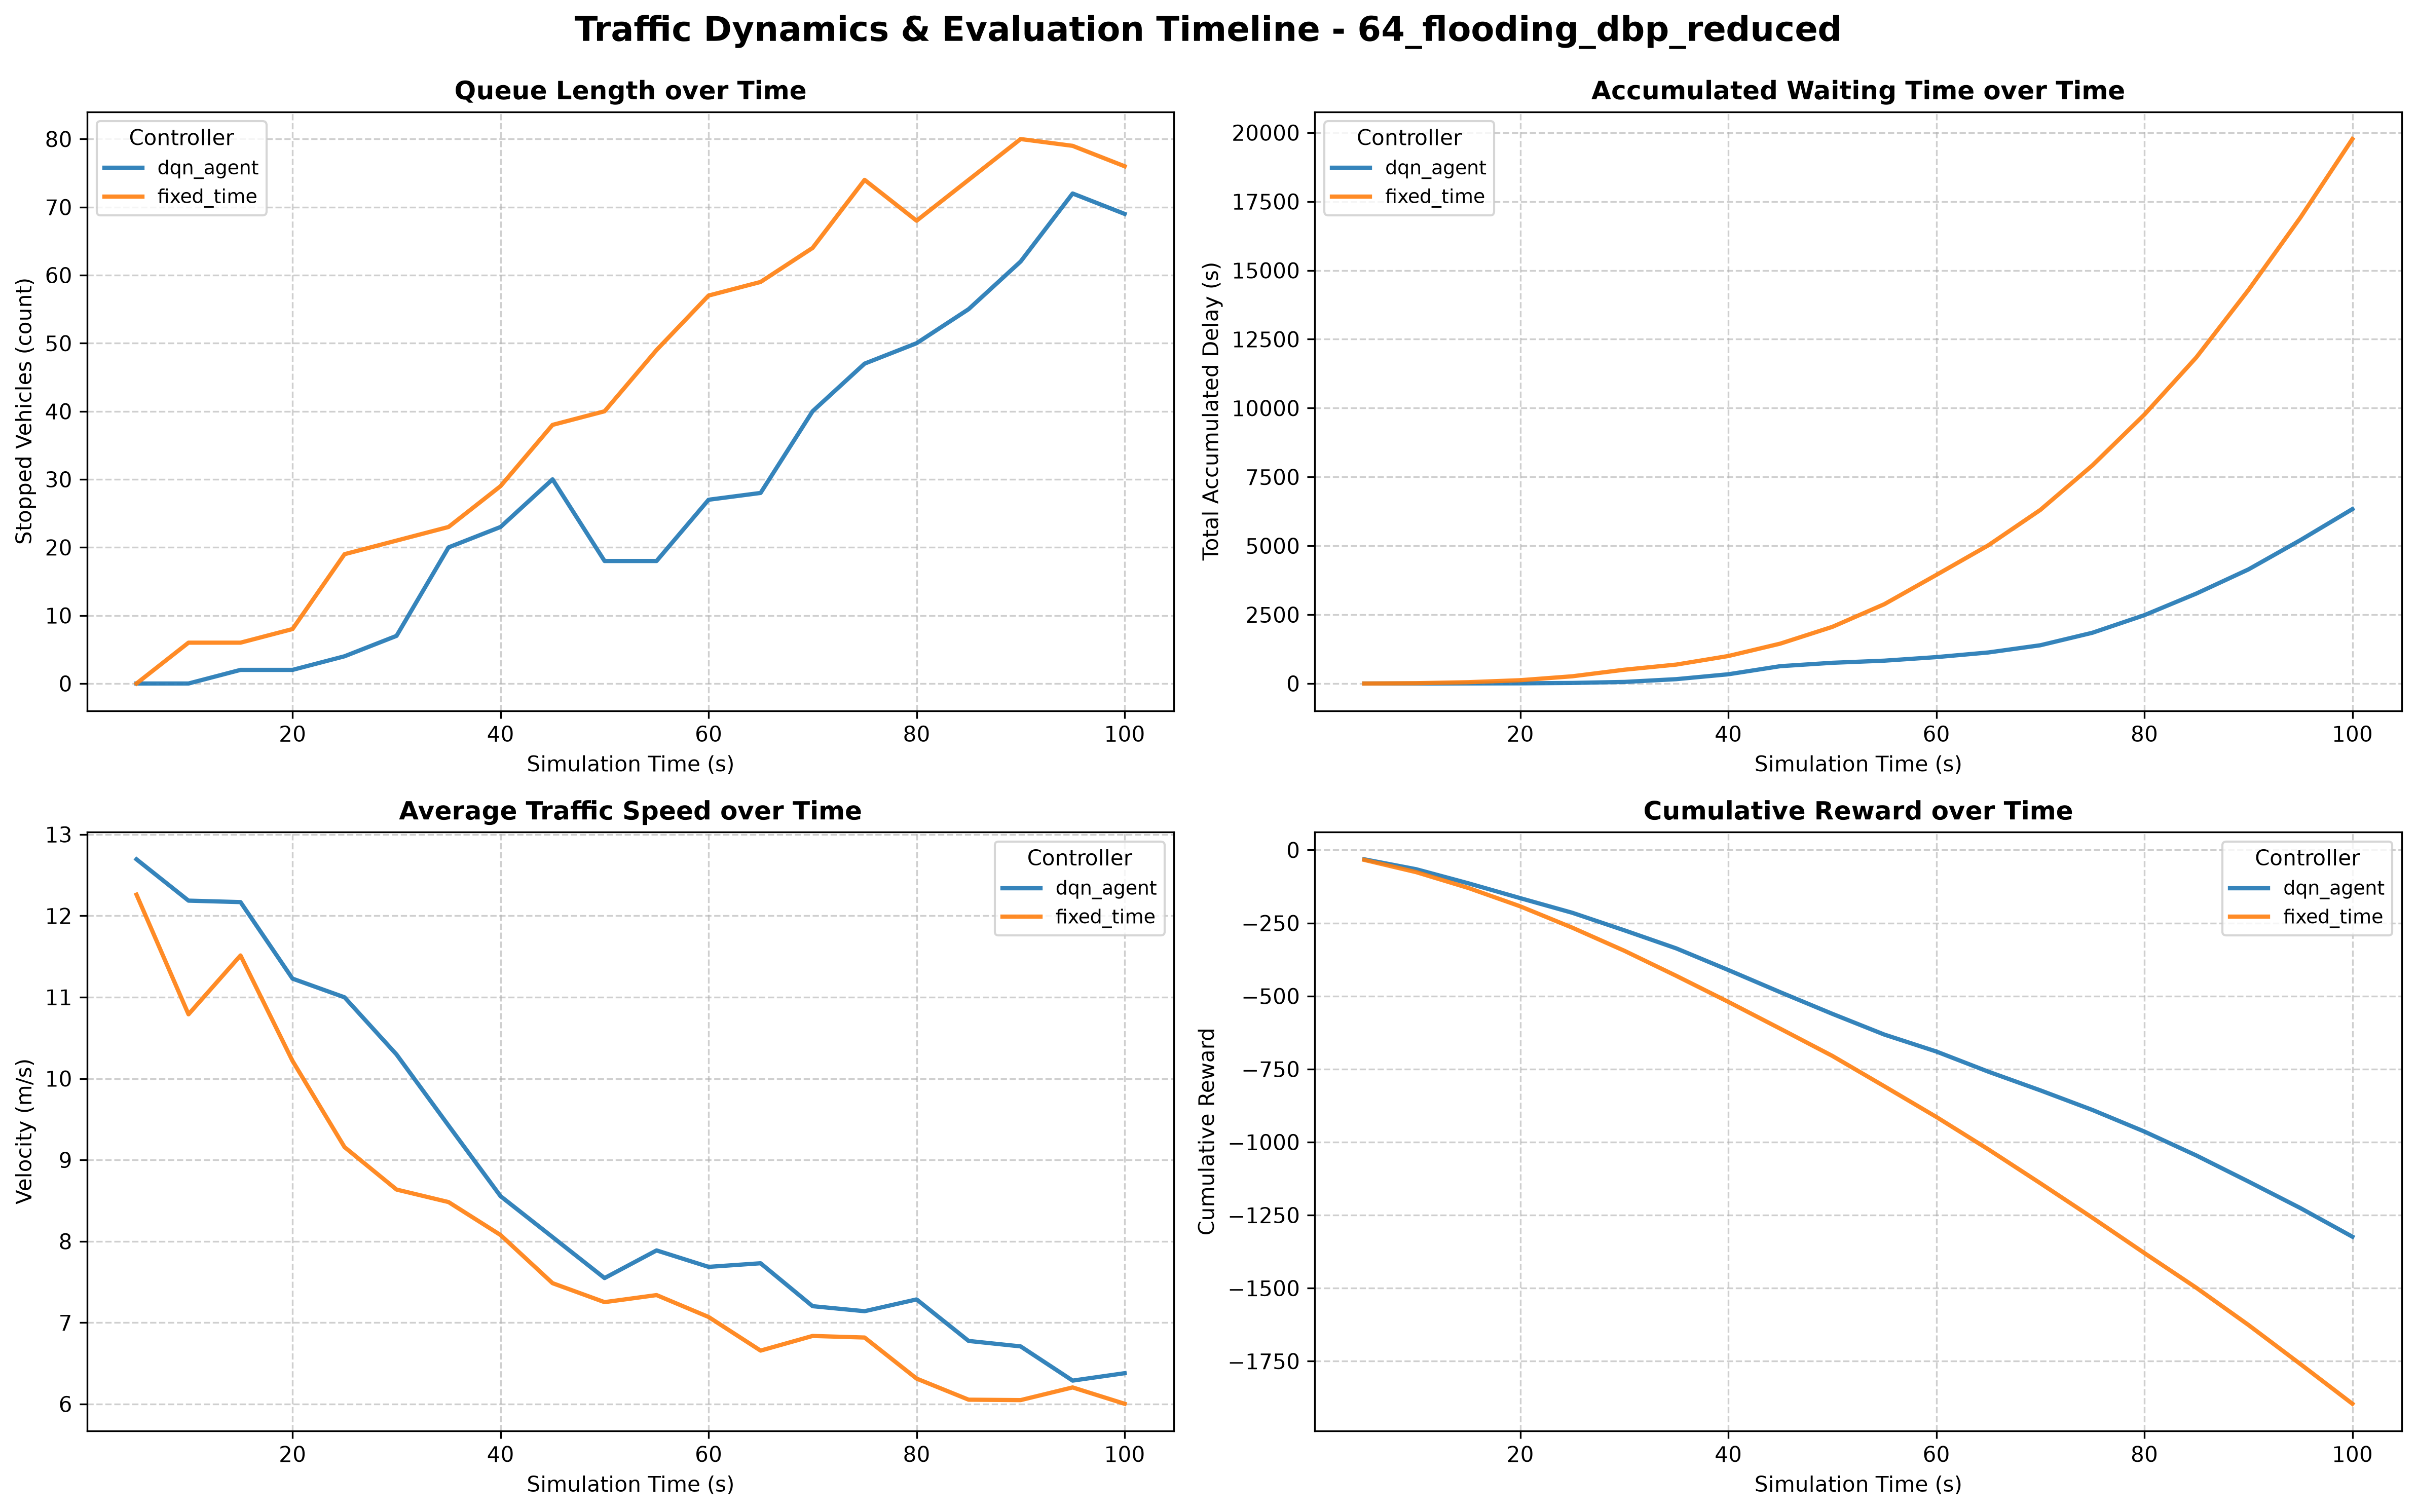
\includegraphics[width=0.92\textwidth]{figures/step_evaluation_dashboard_64.png}
\caption{Four-panel microscopic traffic dynamics timeline on \texttt{64\_flooding\_dbp\_reduced} ($0\text{--}100\,\mathrm{s}$): instantaneous queue length, network-wide accumulated waiting time, average vehicle speed, and cumulative reward.}
\label{fig:step-dashboard-64}
\end{figure*}

In contrast to completed-trip averages, step-level network telemetry shows consistent gains for \texttt{dqn\_agent} across \emph{all six} test scenarios:
\begin{itemize}
\item \textbf{Network-wide accumulated delay:} Total accumulated waiting time at $t=100\,\mathrm{s}$ is lower under \texttt{dqn\_agent} in every scenario, decreasing from a mean of $16{,}813\,\mathrm{s}$ to $8{,}151\,\mathrm{s}$ ($51.52\%$ reduction in aggregate mean delay; $50.31\%$ mean per-scenario reduction), with peak reductions of $75.33\%$ in Scenario~80 and $67.97\%$ in Scenario~64.
\item \textbf{Network speed and reward:} Mean traffic speed is higher under \texttt{dqn\_agent} in all six cases ($9.44$ vs.\ $9.04\,\mathrm{m/s}$, $+4.42\%$), and cumulative reward is consistently higher (less negative) across every scenario ($-1799$ vs.\ $-2163$ on average).
\item \textbf{Safety constraints and runtime:} Both controllers record $0$ minimum-green violations across all episodes, confirming that the \texttt{AllRedTrafficSignal} wrapper enforces $t_{\min}=10\,\mathrm{s}$. The DQN policy averages $0.479\,\mathrm{ms}$ per decision step (range $0.452\text{--}0.529\,\mathrm{ms}$), orders of magnitude faster than the $5\,\mathrm{s}$ control cycle.
\item \textbf{Fuel and emissions:} Aggregate six-scenario mean totals are slightly higher under \texttt{dqn\_agent} for fuel ($12.08 \times 10^6$ vs.\ $12.05 \times 10^6$ units, $+0.30\%$ relative to \texttt{fixed\_time}; $-0.29\%$ mean per-scenario improvement), $\mathrm{CO}_2$ ($37.92 \times 10^6$ vs.\ $37.81 \times 10^6\,\mathrm{mg}$, $+0.30\%$ relative change; $-0.30\%$ mean per-scenario improvement), and $\mathrm{NO}_x$ ($27{,}911$ vs.\ $27{,}451\,\mathrm{mg}$, $+1.67\%$ relative change; $-1.88\%$ mean per-scenario improvement). Scenario-level reductions occur in Scenario~80 (fuel $1.21\%$, $\mathrm{CO}_2$ $1.19\%$) and Scenarios~30/68 ($\mathrm{NO}_x$ $1.29\%$ and $2.70\%$).
\end{itemize}
